\chapter{Introducción}
\label{cap:capitulo1}
\setcounter{page}{1}

\begin{flushright}
\begin{minipage}[]{10cm}
\emph{La creatividad es la inteligencia divirtiéndose}\\
\end{minipage}\\

Albert Eintein\\
%Autor, \textit{Título}\\
\end{flushright}

\vspace{1cm}

%[Párrafo sobre la robótica y la importancia de la exploración espacial]
La robótica es un campo multidisciplinario que se concentra en el diseño,
construcción, programación y operación de robots.
Estos dispositivos electromecánicos, con frecuencia modelados
antropomórficamente o zoomórficamente o animal, están destinados a realizar
tareas de manera autónoma o semiautónoma en una variedad de entornos.
La robótica ha experimentado un rápido crecimiento y expansión desde sus inicios
en la década de 1950, abarcando una amplia gama de aplicaciones en la industria,
la medicina, la exploración espacial y el entretenimiento, entre otras.
La robótica sigue evolucionando y desempeñando un papel cada vez más importante
en nuestra sociedad moderna gracias a los avances constantes en tecnologías como
la inteligencia artificial, los sensores y los actuadores, y ha conformado un
factor crucial en la exploración espacial, que en particular, ha impulsado el
desarrollo de tecnologías que luego se han aplicado en la Tierra, mejorando la
calidad de vida de las personas.
Ejemplos destacados incluyen los sistemas de purificación de agua, los tejidos
avanzados como la viscoelástica y los dispositivos de imágenes médicas como la
resonancia magnética.
Estas innovaciones, así como muchas otras, han proporcionado acceso a agua
potable en regiones remotas, a colchones y almohadas que promueven un mejor
descanso, y a diagnósticos médicos precisos sin radiación nociva.
Así, la investigación espacial no solo expande nuestro conocimiento del
universo, sino que también beneficia directamente a la humanidad en la Tierra.
En este contexto introductorio, se exploran conceptos fundamentales de la
robótica, así como áreas clave que están redefiniendo los límites de la
tecnología, como son la robótica móvil y la robótica de bajo coste.
Estas dos áreas no solo son grandes avances tecnológicos, sino que también
tienen un gran impacto en cómo usamos la tecnología en nuestra vida diaria.
Un ejemplo ilustrativo de la aplicación de la robótica en la exploración
espacial se encuentra en los resistentes robots enviados a diferentes planetas
del sistema solar en busca de datos científicos, como lo evidencian numerosas
misiones científicas.
Esto se puede observar en la Figura \ref{fig:rover}, donde se muestran dos
robots específicamente destinados a Marte por la NASA en 2020.

\begin{figure} [h!]
  \begin{center}
    \includegraphics[width=8cm]{figs/perseverance_and_ingenuity_mars_rover_selfie}
  \end{center}
  \caption{Rover Perseverance y helicoptero Ingenuity de la NASA en Marte.}
  \label{fig:rover}
\end{figure}\

%[TODO] más o menos cada párrafo una imagen en la introducción (con h! es lo mas restrictivo posible).

%[TODO] enlazar los párrafos con su siguiente párrafo.

%[Párrafo sobre la robótica móvil]
La robótica móvil ha emergido como un campo multidisciplinario que fusiona la
ingeniería, la inteligencia artificial y múltiples ramas de la robótica y la
mecatrónica para crear sistemas capaces de moverse y operar en entornos
dinámicos, interactuando con los mismos de manera que reciben información
mediante sensores y aplican cambios en el medio gracias a sus actuadores, todo
ello de manera inteligente debido al software integrado y a su capacidad de
cómputo.
Desde sus inicios, ha sido impulsada por avances significativos en tecnología,
incluyendo sensores y actuadores cada vez más sofisticados, poder de
procesamiento mejorado y algoritmos de control más eficientes.
Estos avances han permitido la aplicación de robots móviles en una amplia gama
de áreas, desde la exploración espacial y submarina hasta la logística
industrial y la atención médica, siendo ya parte indispensable de nuestras vidas
y mejorando su calidad.
En este contexto, la investigación en robótica móvil se centra en desarrollar
sistemas autónomos capaces de navegar de manera segura y eficiente en entornos
desconocidos, adaptarse a cambios imprevistos y realizar tareas complejas de
manera autónoma.
Un ejemplo representativo de este tipo de robots se puede ver en la Figura
\ref{fig:atlas}, donde se pueden observar dos de los robots más desarrollados en
el ámbito móvil, demostrando una gran versatilidad en una variedad de entornos
para ejecuatr una amplia variedad de tareas, desde abrir puertas hasta
transportar cargas de peso, realizar trabajos manuales, o incluso seguir rutinas
de deportivas variadas, que en muchos casos iguala o incluso supera la de los
humanos, dependiendo de la situación especifica.

\begin{figure} [h!]
  \begin{center}
    \includegraphics[width=8cm]{figs/atlas_spot_boston_dynamics}
  \end{center}
  \caption{Robots Spot y Atlas de Boston Dynamics.}
  \label{fig:atlas}
\end{figure}\

%[Párrafo sobre la robótica de bajo coste y en relación con la educación]
La robótica de bajo coste se refiere al desarrollo e implementación de sistemas
robóticos como los descritos anteriormente utilizando componentes y recursos
económicos, con el objetivo de hacer la tecnología robótica más accesible y
asequible para una amplia gama de aplicaciones y usuarios.
Este enfoque busca reducir los costos asociados con la construcción y operación
de robots, empleando materiales económicos, hardware de bajo coste y técnicas
de fabricación eficientes. En el contexto de la robótica móvil, los sistemas de
bajo coste pueden ofrecer soluciones viables para aplicaciones con presupuestos
limitados o despliegues a gran escala, abarcando un papel crucial en áreas como
la educación, la investigación académica, la asistencia social y la exploración
de entornos remotos o peligrosos.
Además de su utilidad práctica, la robótica de bajo coste también promueve la
innovación y el desarrollo de nuevas tecnologías al proporcionar una plataforma
accesible para la experimentación y la creatividad abierta a una amplia
comunidad.
Un ejemplo destacado es el robot Sora-Q visible en la Figura \ref{fig:sora_q},
enviado a la Luna recientemente por la JAXA y desarrollado por una empresa de
juguetería japonesa.
Tras completar su misión, fue comercializado por 150€, lo que ilustra cómo la
tecnología robótica puede volverse accesible para un público más amplio, incluso
después de su participación en misiones espaciales.
La Educación en robotica suele basarse en este tipo de robotica de bajo coste,
ya que las instituciones educativas enfrentan limitaciones presupuestarias que
dificultan la adquisición de sistemas más costosos, por su gran numero de
alumnos, a los que no podrían proveer de sistemas de este calibre de otra
manera.

\begin{figure} [h!]
  \begin{center}
    \includegraphics[width=8cm]{figs/SoraQ_lunar_robot_JAXA}
  \end{center}
  \caption{Sora-Q, robot \textit{low-cost} enviado a la Luna, por Takara Tomy y la JAXA.}
  \label{fig:sora_q}
\end{figure}\

%[Párrafo sobre la educación en robótica en España]
En España, al igual que en el resto de la comunidad europea, la relevancia de la
robótica en el ámbito educativo ha ido ganando terreno en los últimos años,
promoviendo la creatividad, el pensamiento crítico y las habilidades
tecnológicas entre los estudiantes. Desde la década de los 90, se han
implementado programas piloto y competiciones robóticas, como el programa
Robolot (1992), desarrollado por la UPC, las Olimpiadas de Informática (1993),
que incorporaron desafíos relacionados con la programación de robots, así como
la RoboCupJunior (2000), ofreciendo a los estudiantes la oportunidad de diseñar,
construir y programar robots para competir en diferentes categorías.
En las escuelas primarias y secundarias, se ha observado un incremento en los
últimos años en la implementación de programas educativos que incluyen
actividades prácticas de robótica.
Desde alrededor de 2014, dependiendo de la comunidad autónoma de España, se han
introducido programas y asignaturas que incluyen la robótica como parte esencial
del plan de estudios.
Esto brinda a los estudiantes la oportunidad de desarrollar habilidades
tecnológicas avanzadas desde una edad temprana, además de fomentar el trabajo en
equipo y la resolución de problemas complejos, preparándolos para futuras
carreras relacionadas con la tecnología.
Al ser un área introductoria a la robótica se busca simplificar la programación,
utilizando herramientas como placas como Arduino y plataformas como Scratch,
como se muestra en las Figuras \ref{fig:arduino} y \ref{fig:scratch}
respectivamente.

\begin{figure}[h!]
  \centering
  \begin{minipage}{0.45\textwidth}
    \centering
    \includegraphics[height=6cm]{figs/arduino}
    \caption{Arduino.}
    \label{fig:arduino}
  \end{minipage}
  \hfill
  \begin{minipage}{0.45\textwidth}
    \centering
    \includegraphics[height=6cm]{figs/scratch_arduino_code}
    \caption{Código de Arduino en Scratch.}
    \label{fig:scratch}
  \end{minipage}
\end{figure}\

%[Párrafo sobre la educación en relacion con al robótica móvil]
Dicha educación suele basarse también en la robótica móvil, esto se debe al
hecho de que ver el resultado en movimiento genera en los estudiantes una
sensación de motivación, ilusión por aprender y una realización satisfactoria,
lo cual ayuda en gran medida a su aprendizaje.
Las placas utilizadas en el ámbito educativo, mencionadas anteriormente,
resultan ideales para estos propósitos debido a su coste y simplicidad, sin
embargo, también imponen ciertas limitaciones en las capacidades del robot y en
la posibilidad de añadir hardware externo más complejo, y por tanto en la propia
originalidad y aprendizaje de los estudiantes, restringiendo así su creatividad,
innovación y potencial de creación.
A medida que los estudiantes avanzan en sus conocimientos, se encuentran con el
desafío de dar el siguiente paso: la programación de robots utilizando ROS, la
plataforma estándar por excelencia en robótica. Este proceso implica un
considerable escalón de aprendizaje, ya que no solo deben dominar un lenguaje de
programación más complejo, sino que también comprenedr el entorno que
rodea a este \textit{middleware} robótico.
Este entorno incluye aspecto como las comunicaciones, la arquitectura software,
la programación modular u orientada a objetos, algoritmos y estructuras de
datos, entre otros, que suele conllevar decenas de asignaturas individuales en
los grados de robótica de cualquier universidad.
Dicha complejidad se puede ver reflejada en la Figura \ref{fig:ros}, donde se
muestra un esquema simplificado de la arquitectura de ROS y ROS2 que puede
resultar abrumaora para aquellos que se esán iniciando en este ámbito.
Por este motivo, resulta evidente la necesidad de un paso intermedio que pueda
actuar como puente entre estos dos niveles de aprendizaje, el cual podría ser
incorporado, por ejemplo, en el programa educativo del bachillerato tecnológico
o de centros de educación secundaria.
Este nivel intermedio facilitaría la transición entre las habilidades adquiridas
en la enseñanza primaria o secundaria y los requisitos más avanzados de la
universidad en el campo de la robótica.

\begin{figure} [h!]
  \begin{center}
    \includegraphics[width=10cm]{figs/ROS_and_ROS2}
  \end{center}
  \caption{Arquitectura de ROS y ROS2.}
  \label{fig:ros}
\end{figure}\

%[TODO] hacer collage de las imagenes del video para explicar en varios pasos lo mismo que el video.

%[Párrafo sobre la multirobótica]
La multirobótica es un campo de investigación y desarrollo que estudia y
desarrolla sistemas robóticos compuestos por múltiples robots que trabajan en
conjunto para realizar una variedad tareas complejas.
Estos sistemas pueden dividirse las tareas, como la exploración de entornos
desconocidos o la búsqueda y rescate en áreas de difícil acceso.
Al aprovechar la capacidad de múltiples robots para trabajar en conjunto y
complementarse entre sí, la multirobótica tiene como objetivo mejorar la
eficiencia y la robustez de los sistemas robóticos.
En esta disciplina se analizan los principios fundamentales, los problemas
técnicos y las aplicaciones prácticas de la multirobótica en varios contextos.
El trabajo mencionado se puede apreciar en el ejemplo de la Figura
\ref{fig:multirobots}, en la cual están realizando una tarea de búsqueda,
mediante la división de un área, probablemente desconocida.

\begin{figure} [h!]
  \begin{center}
    \includegraphics[width=8cm]{figs/multirobotics_in_search_and_rescue}
  \end{center}
  \caption{Múltiples robots durante una operacion de búsqueda y rescate.}
  \label{fig:multirobots}
\end{figure}\

%[Párrafo sobre multirobótica en educación].
En el ámbito educativo, la multirobótica ofrece una oportunidad única para
involucrar a los estudiantes en actividades prácticas y colaborativas.
Al trabajar con sistemas multirobot, los estudiantes no solo adquieren
conocimientos sobre programación, control y mecánica de robots, sino que también
exploran conceptos como son las telecomunicaciones entre robots, la coordinación,
la planificación y asignación de tareas ocn o sin prioridades, la localización y
navegación conjunta, así como la seguridad que se requiere para evitar
colisiones entre ellos.
Además, la multirobótica proporciona un entorno de aprendizaje dinámico y
estimulante que despierta aún más la curiosidad y la creatividad de los
estudiantes, preparándolos para enfrentar los desafíos del mundo tecnológico en
constante evolución. Se puede ver un ejemplo de los robots educativos de nuestro
laboratorio de robótica de la URJC en la Figura \ref{fig:robots_education}.

\begin{figure} [h!]
  \begin{center}
    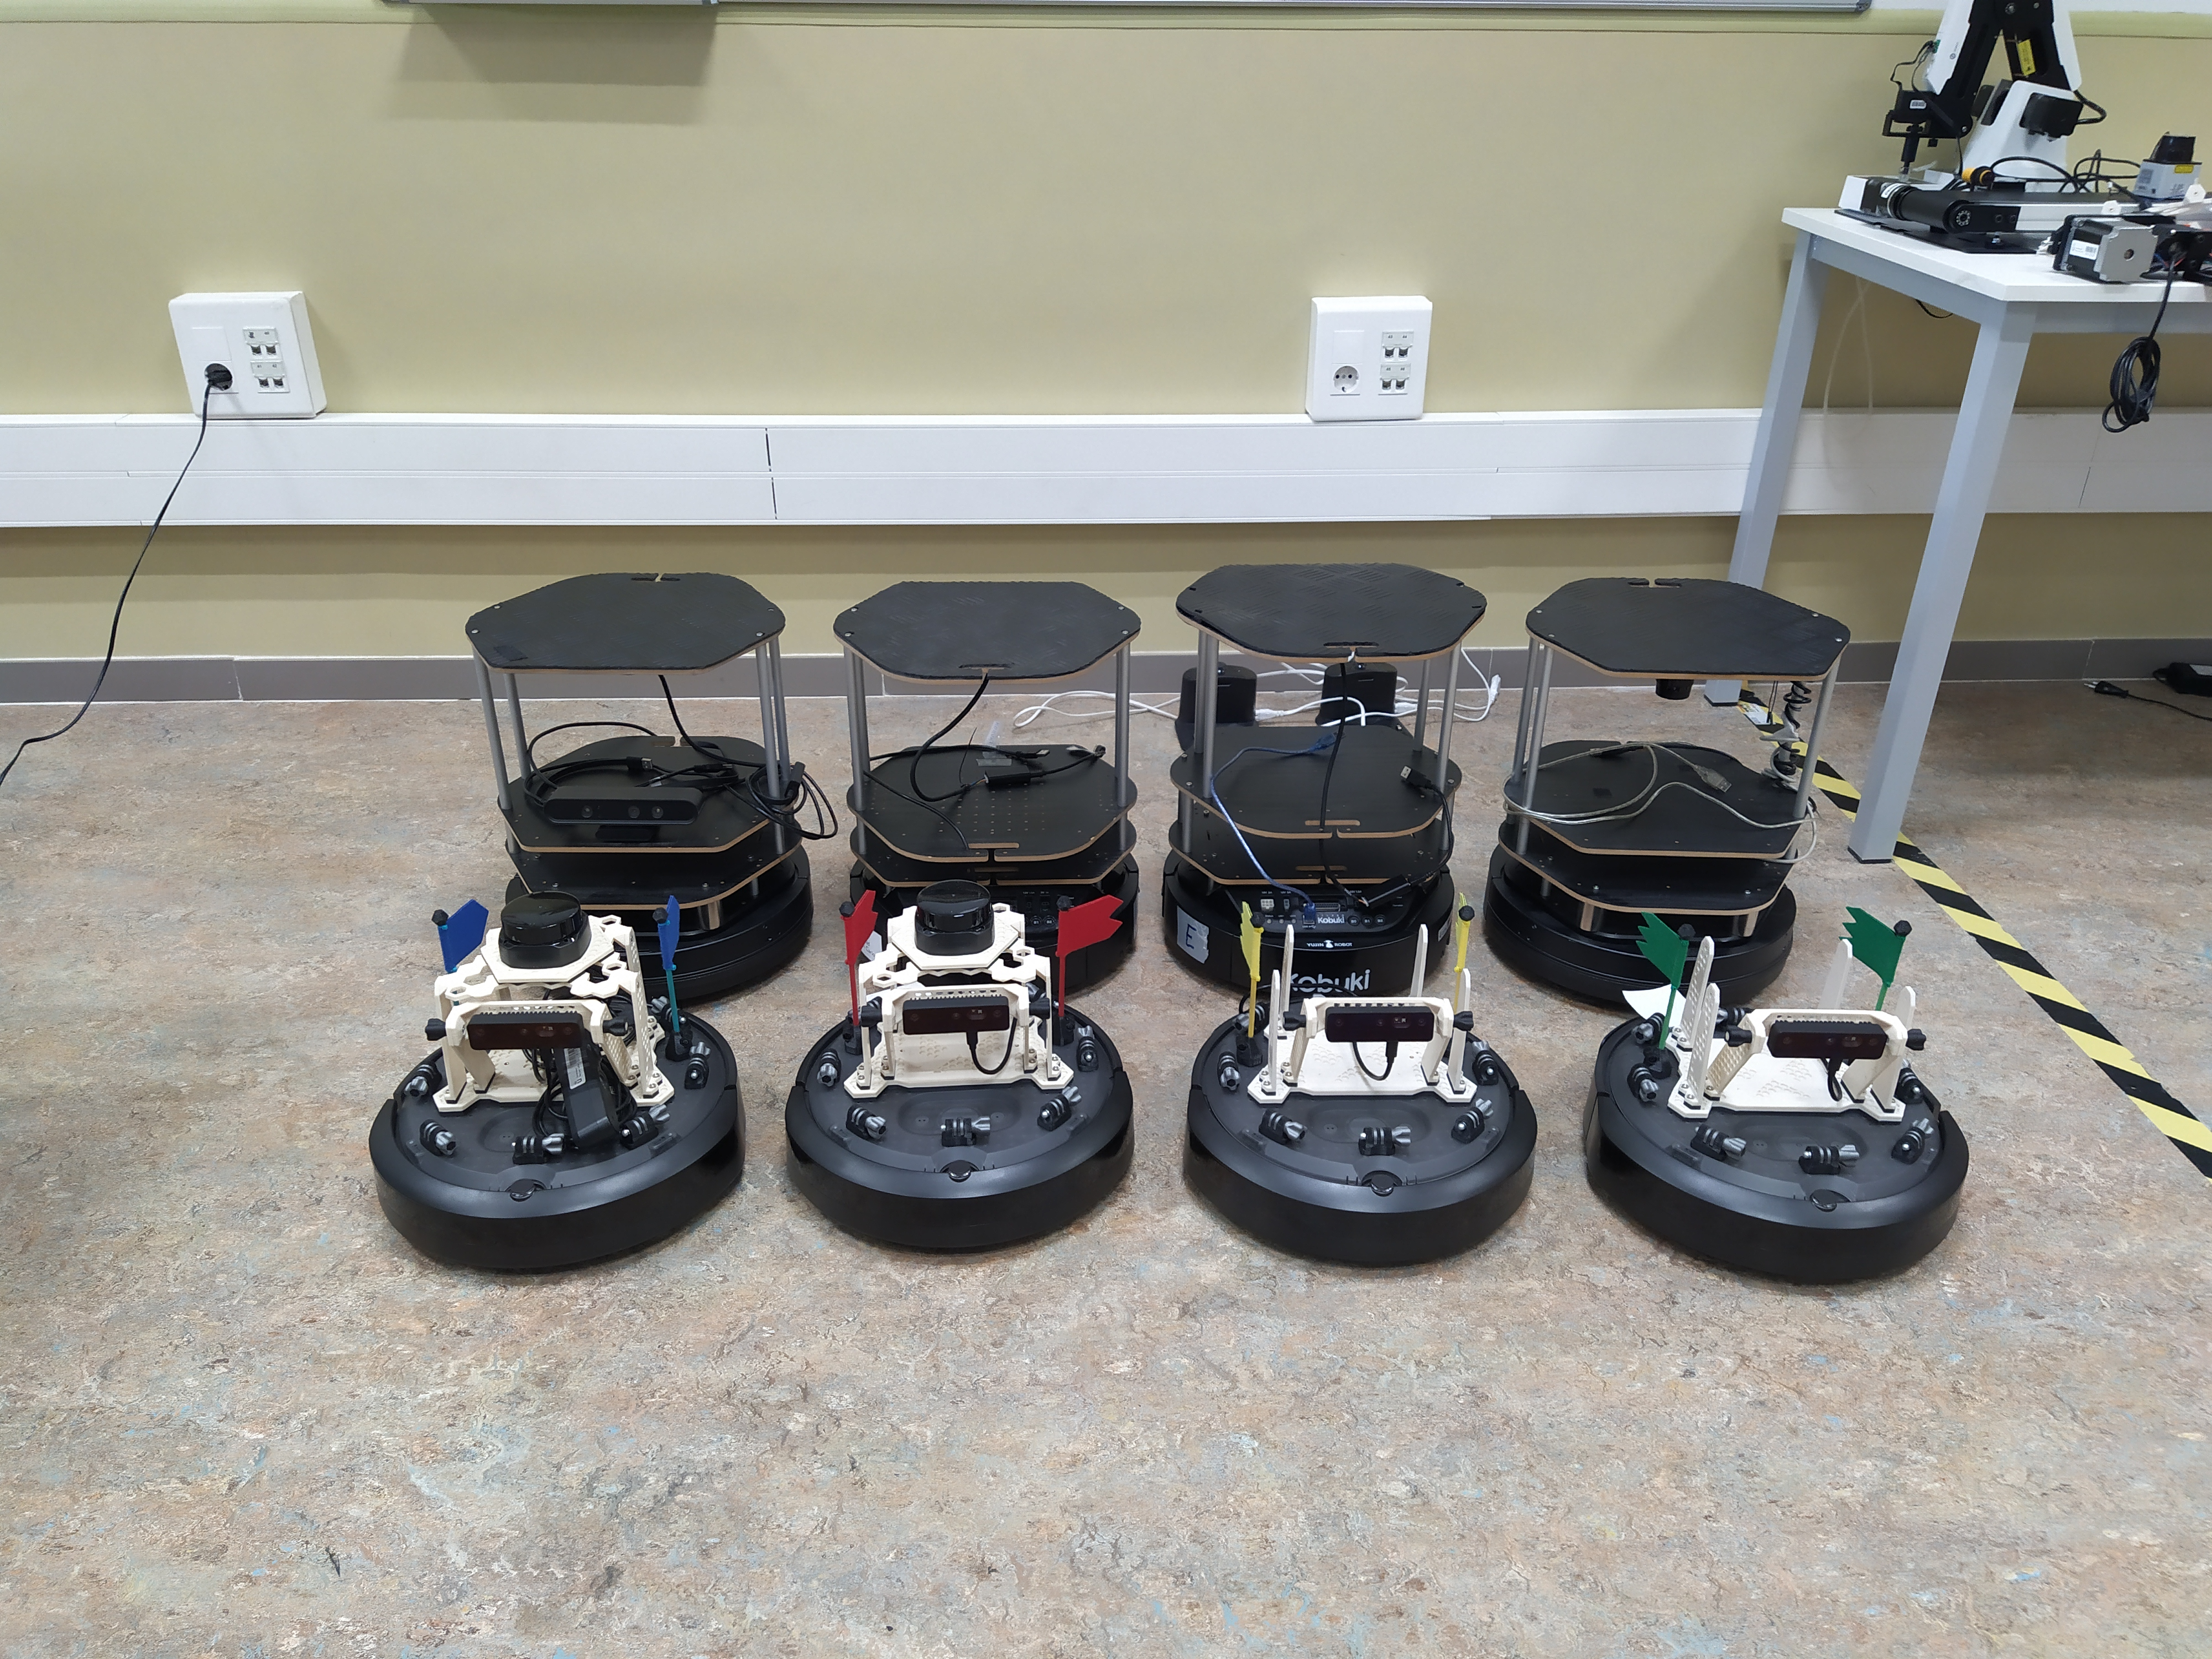
\includegraphics[width=8cm]{figs/multirobotics_education}
  \end{center}
  \caption{Múltiples robots educativo, modelos Turtlebot 2 (arriba) y 4 (abajo).}
  \label{fig:robots_education}
\end{figure}\

%[Párrafo sobre las telecomunicaciones entre robots]
Las mencionadas telecomunicaciones entre robots son fundamentales en la
multirobótica, ya que garantizan una comunicación rápida, optima,
eficiente y ordenada entre los distintos dispositivos, permitiendo de esta
manera un correcto desempeño de la funcionalidad en cuestión.
Sin embargo, este proceso puede enfrentarse a desafíos como la congestión de la
red, y la consecuente pérdida de mensajes, que pueden ser críticos para el
correcto funcionamiento de los robots.
Por este motivo es crucial gestionar cuidadosamente la cantidad de robots y
mensajes generados, minimizándolos para optimizar el rendimiento del sistema y
evitando de esta manera un cuello de botella.
%[TODO] añadir la frase "una de las empresas mas importantes es ZettaScale
%Technology..." para dar un ejemplo introductorio de la empresa, en vez de poner
%que es la mas importante directamente. No ha yque cerrarse en ese aspecto.
%En este aspecto, una de las empresas más importantes del sector es ZettaScale
%Technology, desarrolladora de CyclondeDDS, una de las mejores implementaciones
%de RMW de DDS y con las mejores prestaciones, creadora de Zenoh, el protocolo de
%comunicación que más fuerza está tomando en robótica en estos últimos años,
%habiendo sido su último hito, el comunicad oficial de que Zenoh será la proximo
%RMW de ROS2.
%Esta empresa también es creadora de Zenoh-Flow, un \textit{middleware} para la
%programación de flujos de datos que utiliza Zenoh como protocolo de
%comunicaciones.
%También tienen un puente para comunicar DDS con Zenoh, el
%\textit{zenoh-bridge-dds}, por lo que con todas estas herramientas organizadas y
%configuradas de la manera correcta se pueden programar data-flows que funcionen
%en ROS2, eliminando toda la complejidad de este, pero dejando la posibilidad de
%seguir usando sus nodos.

%[Párrafo sobre flujos de datos y comportamiento reactivo mas simple para educación]
Mantener un flujo de datos correcto es fundamental para solventar los problemas
de telecomunicaciones mencionados en el desarrollo de sistemas de multirobótica.
Además, simplifica el desarrollo del software al proporcionar una clara visión
de la dirección, el origen y el destino de los datos en cada momento.
Esto permite dividir el programa en partes claramente diferenciadas, normalmente
llamadas nodos, modularizándolo y dando lugar a la división del problema último
en varios problemas más simples y fáciles de atajar.
Como resultado, el desarrollo se vuelve un proceso más sostenible y escalable, y
por tanto, más fácil de llevar a cabo por los estudiantes.

%La educación en robótica se basa en la robótica de bajo coste, normalmente en
%placas como Arduino o similares, las cuales son ideales para este uso, y a su
%vez limitan la capacidad del robot en cuestión y el hardware que se puede usar y
%consecuentemente limitan la creatividad y el aprendizaje de los niños. Una vez
%se llega a un cierto nivel de conocimientos, el siguiente paso suele ser la
%programación de robots con ROS2, donde existe un gran escalon de aprendizaje.
%Este trabajo busca simplificar el desarrollo del software en ROS2 y así reducir
%dicho escalón, para hacer más fácil este desarrollo, dando la posibilidad de
%crear aplicaciones robóticas más complejas para robots más completos y que
%permanecen dentro de la categoría de robots de bajo coste y por tanto siguen
%siendo asequibles para instituciones como colegios o institutos.\\

%Escribe aquí un párrafo explicando brevemente lo que vas a contar en este capítulo. En este primer capítulo, el de introducción, se trata de dar un contexto amplio y atractivo del trabajo. Comienza hablando de un contexto general y acaba hablando del contexto más específico en el que se enmarca el proyecto. Es el capítulo idóneo para incluir todas las referencias bibliográficas que hayan tratado este tema; suponen un fuerte respaldo al trabajo.\\

\section{Problemas de ROS en relación con el aprendizaje}
\label{sec:miseccion} % etiqueta para luego referenciar esta sección

%\section{Problemas de ROS en relación con el aprendizaje}
%\label{sec:miseccion} % etiqueta para luego referenciar esta sección

%ROS es el estándar en robótica para la programación de robots, pero tiene un
%problema y es el gran escalón de aprendizaje que existe cuando se pasa de una
%placa simple como arduino, a robots más complejos con máquinas integradas como
%las placas Raspberry Pi o un ordenador portátil directamente. Esto conlleva a una gran
%diferencia entre la robótica que se enseña en los colegios e institutos a la que
%se ebnseña en universidades, y es debido precisamente a la complejidad de código
%y enseñanza de ROS, para los cuales, se requiere incluso de varias asignaturas.
%Por eso en este trabajo se pretende incorporar un paso intermedio en este gran
%escalón.
%
%La propia naturaleza de este \textit{middleware} robótico nos obliga a programar
%nodos que se ejecutan iterativamente en bucle, sin necesidad de generar una
%topología de red concreta para saber de donde vienen o a donde van los datos, lo
%que puede ser un poco complicado de entender a primera vista para los niños.\\
%
%Además de este problema, existe otro relacionado con la congestión de red: los
%nodos de ROS2 se comunican a través de DDS, un protocolo de comunicaciones que
%genera una gran cantidad de mensajes de \textit{Discovery}, lo que conlleva
%consecuentemente a la generación de congestión de la red, y dificulta de esta
%manera la programacion de aplicaciones multirobóticas, que son un posible
%siguiente paso en la enseñanza de la robotica, para entender las comunicaciones
%entre los distintos robots.\\
%
%Este trabajo prentende solucionar tanto el problema del escalón de aprendizaje,
%suponiendo un paso intermedio en la enseñanza de la robótica, y el problema de
%la congestión de red generala por DDS, suponiendo una posible solución a la
%misma.\\
%
%El problema de la congestión se soluciona usando otro protocolo llamado Zenoh,
%con mejores prestaciones que DDS, y la simplicidad del código de ROS2, se ha
%conseguido gracias al uso de un \textit{framework} llamado Zenoh-Flow, que
%funciona sobre el protocolo mencionado y el cual le da nombre. Este
%\textit{framework} está pensado para la programación de flujos de datos,, por lo
%que hay que definir primero un flujo de datos que luego seguiran los nodos,
%activando su iteración al momento de recibir un dato, generando de esta manera
%un flujo de datos que pasa de nodo a nodo, a diferencia de ROS.\\
%
%La implementación conjunta con ROS es posible gracias a que Zenoh-flow permite
%serializar los datos que se quieren enviar, y existe un bridge que los traduce
%de Zenoh a DDS para que los nodos de ROS2 entiendan dicha información. Es por
%este motivo, que si se serializan los mensajes de la misma manera que se hace
%internamente en ROS2, se pueden seguir utilizando nodos ya implementado en ROS2,
%como puede ser la navegación.\\

%En los textos puedes poner palabras en \textit{cursiva}, para aquellas expresiones
%en sentido \textit{figurado}, palabras como \textit{robota}, que está fuera del
%diccionario castellano, o bien para resaltar palabras de una colección:
%\textit{(a)} es la primera letra del abecedario, \textit{(b)} es la segunda, etc.\\

%Al poner las dos líneas del anterior párrafo, este aparecerá separado del anterior. Si no las pongo, los párrafos aparecerán pegados. Sigue el criterio que consideres más oportuno.

\section{Segunda sección}
\label{sec:segundaseccion}

No olvides incluir imágenes y referenciarlas, como la Figura \ref{fig:roomba}.

%\begin{figure} [h!]
%  \begin{center}
%    \includegraphics[width=8cm]{figs/roomba}
%  \end{center}
%  \caption{Robot aspirador Roomba de iRobot.}
%  \label{fig:roomba}
%\end{figure}\

Ni tampoco olvides de poner las URLs como notas al pie. Por ejemplo, si hablo de la Robocup\footnote{\url{http://www.robocup.org}}.

\subsection{Números}
\label{sec:subseccion}

En lugar de tener secciones interminables, como la Sección \ref{sec:miseccion}, divídelas en subsecciones.

Para hablar de números, mételos en el entorno \textit{math} de \LaTeX, por ejemplo, $1.5Kg$. También puedes usar el símbolo del Euro como aquí: 1.500\euro.

\subsection{Listas}

Cuando describas una colección, usa \texttt{itemize} para ítems o \texttt{enumerate} para enumerados. Por ejemplo:

\begin{itemize}
 \item \textit{Entorno de simulación.} Hemos usado dos entornos de simulación: uno en 3D y otro en 2D.
 \item \textit{Entornos reales.} Dentro del campus, hemos realizado experimentos en Biblioteca y en el edificio de Gestión.
\end{itemize}\

\begin{enumerate}
 \item Primer elemento de la colección.
 \item Segundo elemento de la colección.
\end{enumerate}\

\paragraph{Referencias bibliográficas}
\label{sec:referencias}

Cita, sobre todo en este capítulo, referencias bibliográficas que respalden tu argumento. Para citarlas basta con poner la instrucción \verb|\cite| con el identificador de la cita. Por ejemplo: libros como \cite{vega12e}, artículos como \cite{vega19b}, URLs como \cite{vega19a}, tesis como \cite{vega18b}, congresos como \cite{vega18a}, u otros trabajos fin de grado como \cite{vega08b}.

Las referencias, con todo su contenido, están recogidas en el fichero \texttt{bibliografia.bib}. El contenido de estas referencias está en formato \texttt{BibTex}. Este formato se puede obtener en muchas ocasiones directamente, desde plataformas como \texttt{Google Scholar} u otros repositorios de recursos científicos.

Existen numerosos estilos para reflejar una referencia bibliográfica. El estilo establecido por defecto en este documento es APA, que es uno de los estilos más comunes, pero lo puedes modificar en el archivo \texttt{memoria.tex}; concretamente, cambiando el campo \verb|apalike| a otro en la instrucción \verb|\bibliographystyle{apalike}|. 

\

\

\

Y, para terminar este capítulo, resume brevemente qué vas a contar en los siguientes.
